\documentclass{standalone}
\usepackage[T1]{fontenc}
\usepackage[utf8]{inputenc}
\usepackage{pgf,tikz}
\usepackage{setspace}
\usepackage{pgfplots}
%\pgfplotsset{compat=1.9}


\begin{document}


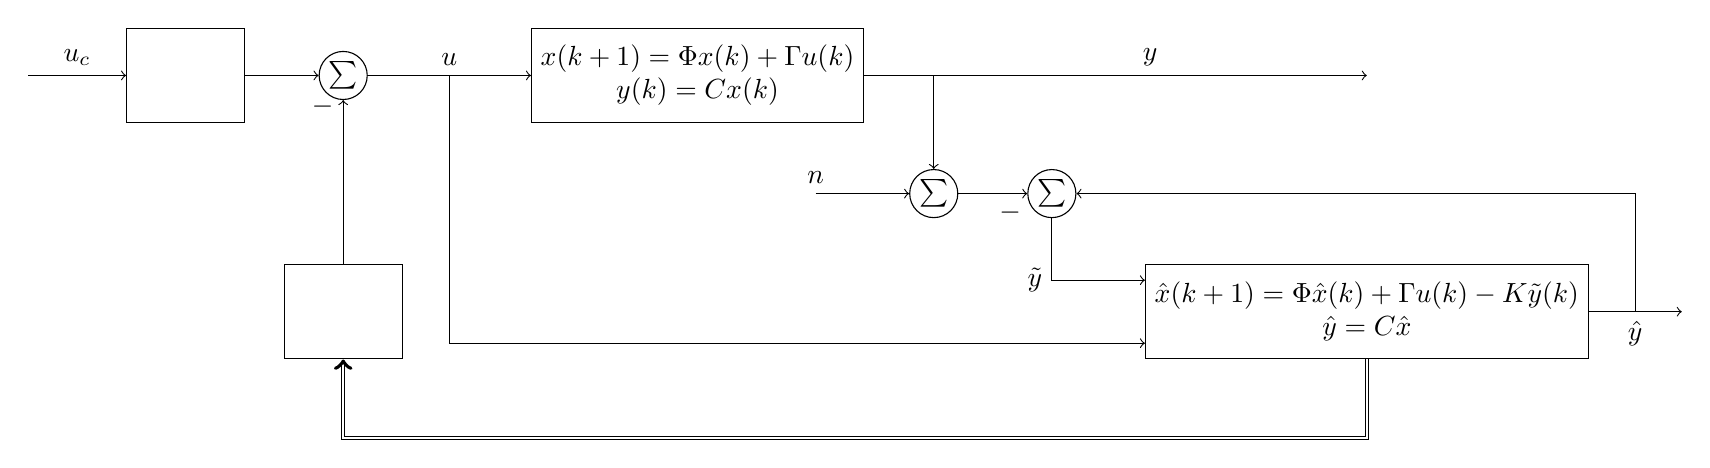
\begin{tikzpicture}[
    node distance=2cm, block/.style={rectangle, draw, minimum height=12mm, minimum width=15mm}, sumnode/.style={circle, draw, inner sep=1pt}]

  \node[coordinate] (input) {};
  \node[block, right of=input] (inputgain) {$$}; %l_0
  \node[sumnode, right of=inputgain] (sum) {$\sum$};
  \node[block,right of=sum, node distance=45mm, align=center] (plant) {$x(k+1) = \Phi x(k) + \Gamma u(k)$\\$y(k) = Cx(k)$};
  \node[coordinate, right of=plant, node distance=30mm] (measure) {};
  \node[coordinate, right of=measure, node distance=55mm] (output) {};
  \node[block,below of=output, node distance=30mm, align=center] (observer) {$\hat{x}(k+1) = \Phi \hat{x}(k) + \Gamma u(k) - K \tilde{y}(k)$\\ $\hat{y} = C \hat{x}$};
  \node[sumnode,below of=measure, node distance=15mm] (sumnoise) {$\sum$};
  \node[sumnode,right of=sumnoise, node distance=15mm] (sumobs) {$\sum$};
  \node[coordinate, left of=sumnoise, node distance=15mm] (noise) {};
  \node[block, below of=sum, node distance=30mm] (feedbackgain) {$$}; % L
  \node[coordinate, right of=observer, node distance=40mm] (observeroutput) {};

  \draw[->] (input) -- node[above] {$u_c$} (inputgain);
  \draw[->] (inputgain) -- node[above] {} (sum);
  \draw[->] (sum) -- node[above] (umeas) {$u$} (plant);
  \draw[->] (plant) -- (measure) -- node[above] {$y$} (output);
  \draw[->] (measure) -- (sumnoise);
  \draw[->] (noise) --  node[at start, above] {$n$} (sumnoise);
  \draw[->] (sumnoise) -- node[below, near end] {$-$}(sumobs);
  \draw[->, double ] (observer.south) |- ++(0,-1cm) -| (feedbackgain);
  \draw[-> ] (feedbackgain) -- (sum) node[left, pos=0.96] {$-$};
  \draw[-> ] (observer) -- node[below] (obsmeas) {$\hat{y}$} (observeroutput);

  \draw[->] (obsmeas) |- (sumobs);
  \draw[<-] (observer.west) ++ (0, 4mm) -| node[left] {$\tilde{y}$} (sumobs);
  \draw[<-] (observer.west) ++ (0, -4mm) -| (umeas);
  
\end{tikzpicture}
\end{document}


